\headline{{\textbf{\Large\sffamily MEP Session Two:}}\\
          {\textbf{\large\sffamily Mastering the Art of the Repot}}}
\phantomsection
\label{2026-01-workshop-mep}

\topic{Evolution of the Programme}
\noindent
Building on the momentum of our December launch, the second meeting of the Member Education Programme (MEP) on Saturday, 17th January, proved that this initiative is fast becoming the heartbeat of our club’s educational calendar.
We owe a debt of gratitude to our volunteer instructors—Tony Ulatowski, Chris Durne, and Nick Lloyd—for their meticulous organisation.
A special mention must also go to Tina Todd; while she modestly insists she is a student like the rest of us, her authoritative yet friendly guidance has become an indispensable part of the MEP experience.

This session saw a slight shift in format, introducing a more structured pedagogical approach.
We began with a plenary session led by Tony, who outlined the fundamental principles of tree positioning within a container.
While Tony’s attempt to use the wall as a makeshift blackboard was met with some technical resistance from the masonry, the lesson was clear: successful repotting is as much about aesthetic balance and future growth as it is about fresh soil.

\medskip
\topic{Hands-on Mastery and New Talents}
\noindent
Following the theory, the room erupted into a hive of activity.
For many, the focus was the critical task of winter repotting and root pruning.
The atmosphere was a perfect blend of intense concentration and the spirited banter that defines the Twickenham family.

Notably, the session served as a training ground for the upcoming New Talent Competition.
David Fishwick arrived with a "boot full of collected silver birch" and a vision, which he transformed into a stunning \textit{kabudachi} (clump style) composition on a slab.
Similarly, Victoria Miquel showed her competitive intent, working on a juniper provided by Nick Lloyd.
Under Chris Durne’s watchful eye, Victoria explored advanced styling techniques, proving that the MEP is providing the exact platform needed for our members to "level up" their skills.

\topic{Celebrating Success: The Novice Trophy}
\noindent
The morning was punctuated by a moment of celebration as Tony Ulatowski presented the \textbf{Novice Tree of the Month Overall 2025} trophy to a visibly shocked Martin Redfern.

\vfill
\begin{minipage}[b]{0.45\textwidth}
    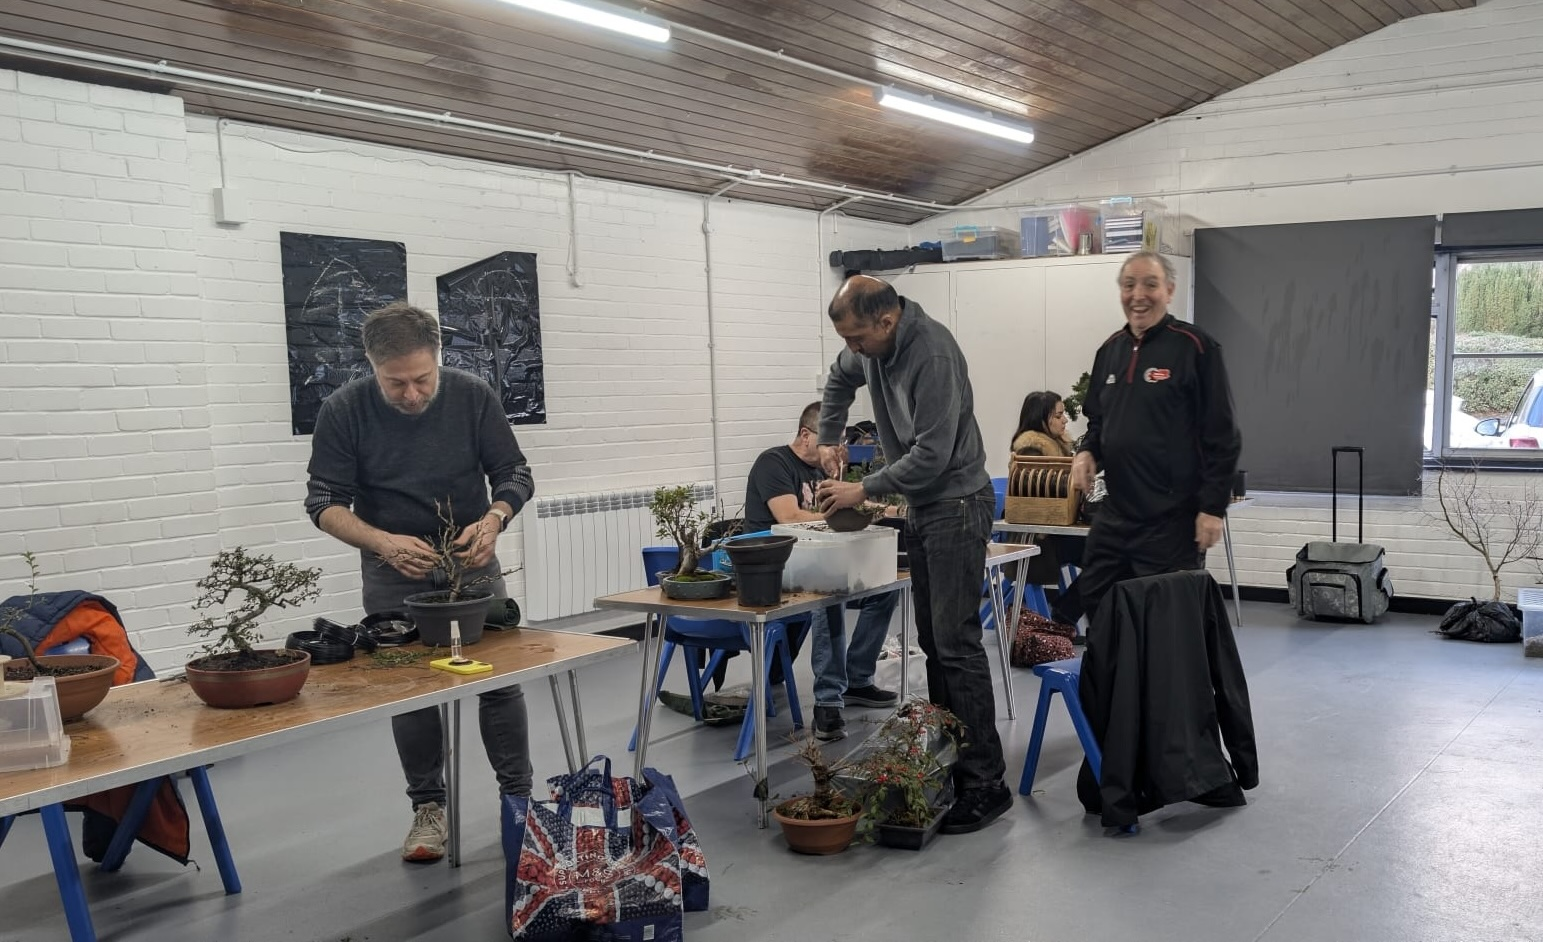
\includegraphics[angle=0,origin=c,width=1.0\textwidth]{2026_01/res/workshop_mep2_working_hard}
    \centerline{\emph{Instructors helping students turning theory into practice.}}
\end{minipage}
\columnbreak

\noindent
Having missed the January club night, Martin was finally able to claim his prize.
The trophy is his to polish and cherish for the year—a tangible reminder of the progress that can be made through dedication and the support of the club.

\medskip
\topic{Voices from the Bench}
\noindent
The feedback gathered during our post-session debrief and via the club chat has been overwhelmingly positive, highlighting the psychological impact of these workshops.

\textbf{Martin Redfern} reflected on his cotoneaster’s first repot in four years: \emph{"With the help and guidance from Tony, I had the confidence to take on the job. The tree is now in a much freer draining mix and the lower trunk is exposed—it's a lot better for the show."}
\textbf{Stefano Bragaglia} noted the strategic value of the sessions: \emph{"The real value lies in understanding when and why to use techniques. The Saturday slot makes it much easier to focus than on a club evening."}

\textbf{Victoria Miquel} described the workshop as ``very valuable,'' while \textbf{Riz Mizra} appreciated the safe space for learning: \emph{``It's a wonderful forum to gain confidence. I found it easier to ask `silly questions' here.''}
\textbf{Nick Lloyd} perhaps summed it up best, stating that the MEP is simply about \emph{``providing people with the platform to gain confidence in their own abilities.''}

\medskip
\topic{Looking Ahead: February and Beyond}
\noindent
The journey continues on \textbf{Saturday, 28th February 2026} at the Whitton Community Centre.
This session will remain focused on the intricacies of repotting and positioning—skills that are foundational to the health and beauty of our trees.

If you have not yet secured your place, please contact \textbf{Tony Ulatowski} or \textbf{Chris Durne} via WhatsApp immediately.
These sessions are filling up faster than a pot with fresh akadama, and you won’t want to miss out on the final repotting workshop of the season.

\medskip
\topic{Conclusion}
\noindent
The second MEP meeting was more than just a workshop; it was a demonstration of our collective growth
By removing the ``fear factor'' and replacing it with shared wisdom, we are ensuring that the art of bonsai remains accessible and thriving in Twickenham.

\vfill
\closearticle
\begin{minipage}[b]{0.45\textwidth}
    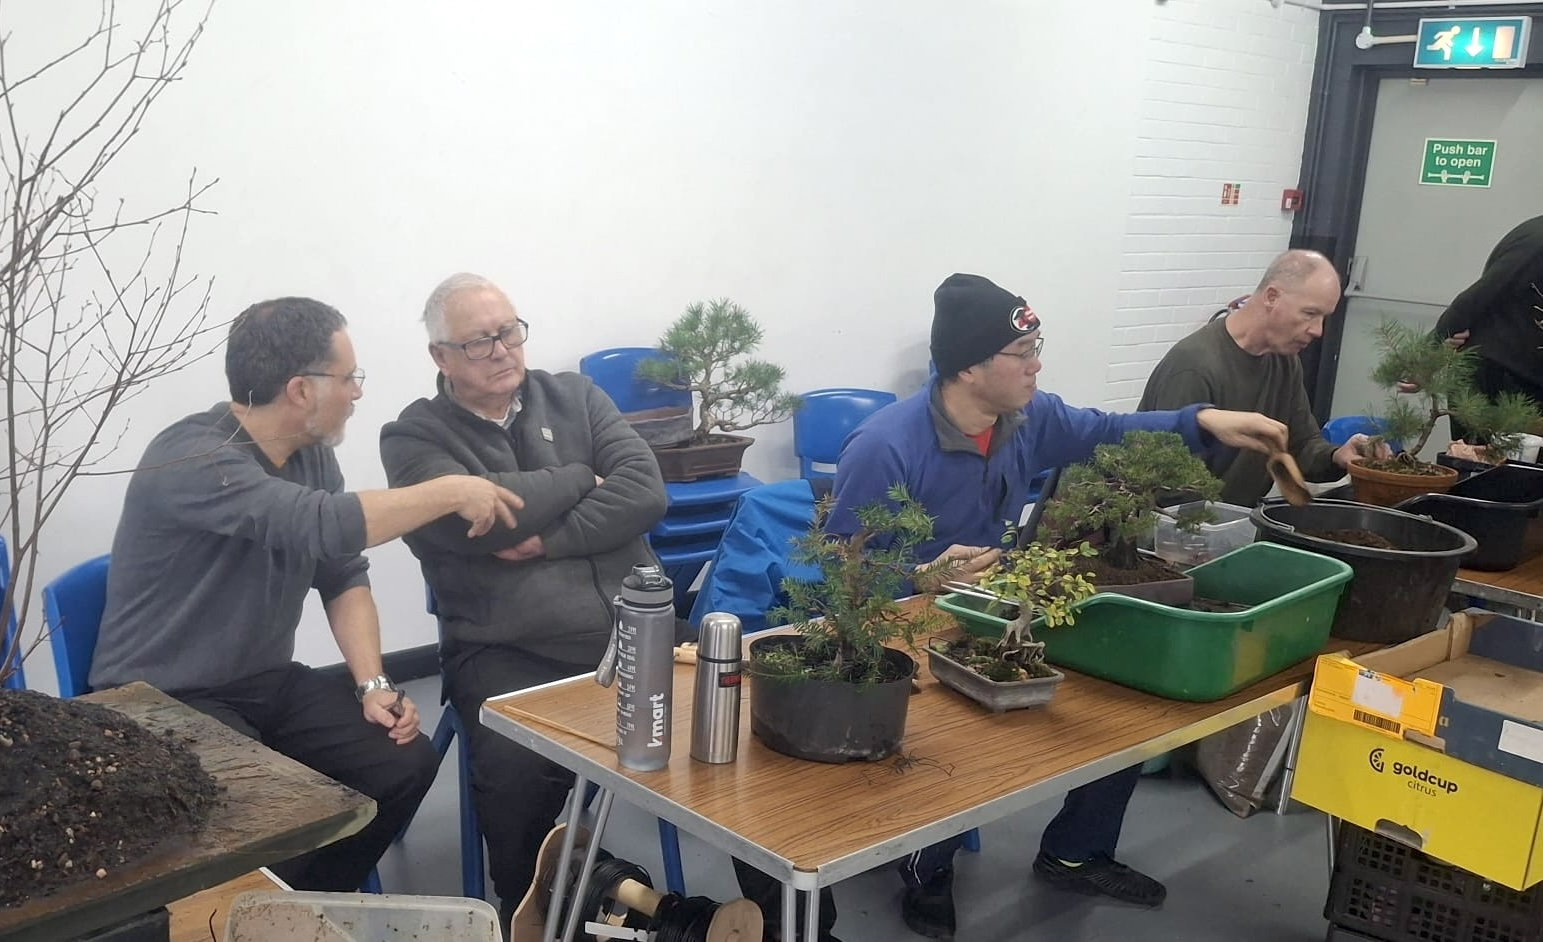
\includegraphics[angle=0,origin=c,width=1.0\textwidth]{2026_01/res/workshop_mep2_general_vibe}
    \centerline{\emph{The MEP as a way to gain confidence in own skills.}}
\end{minipage}

\columnbreak

\begin{minipage}[b]{0.45\textwidth}
    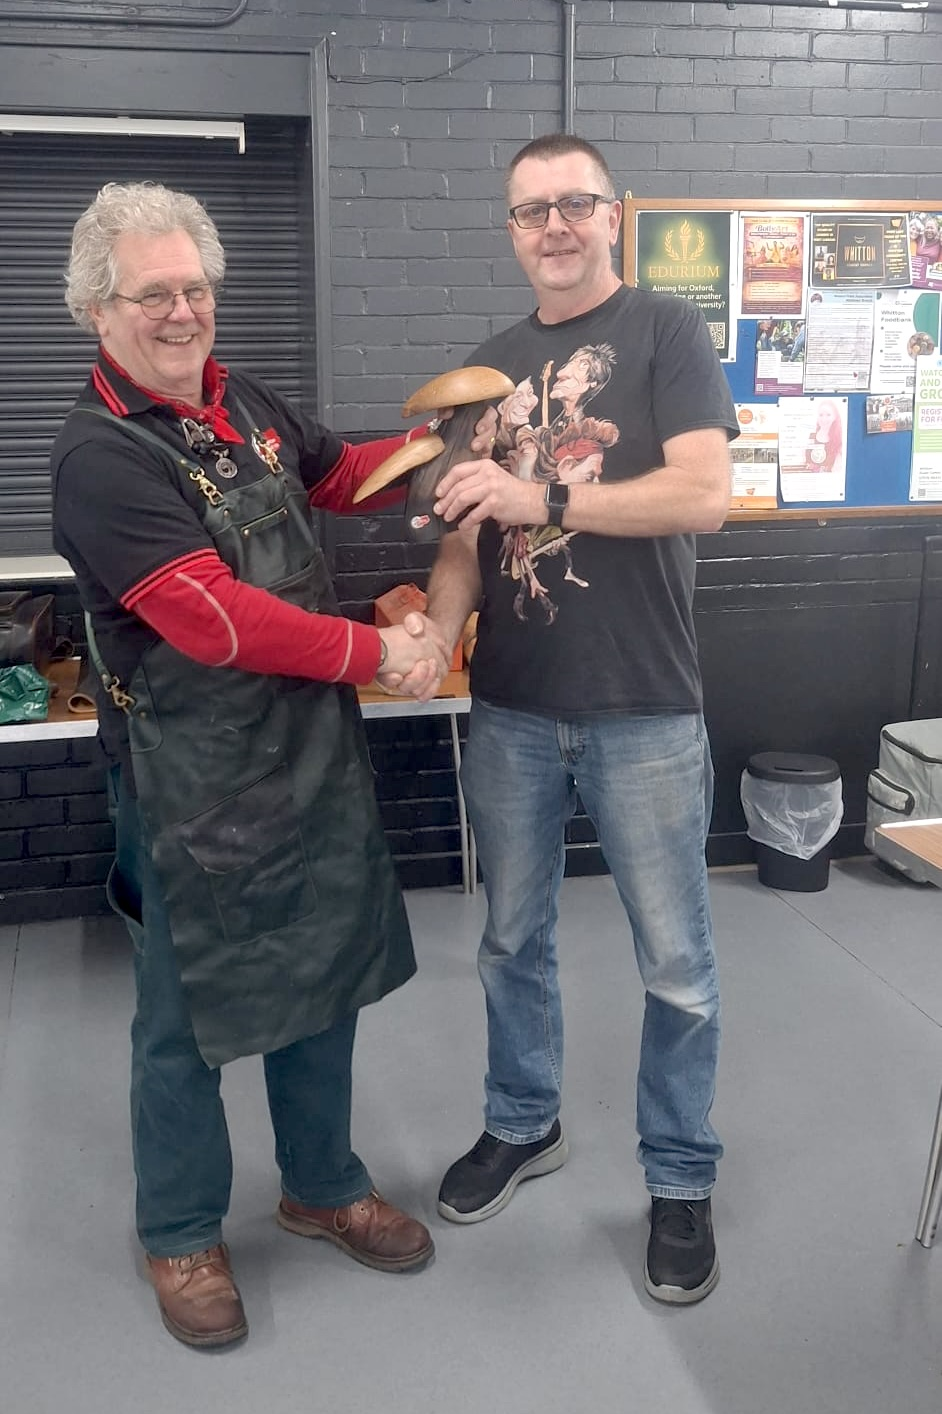
\includegraphics[angle=0,origin=c,width=1.0\textwidth]{2026_01/res/workshop_mep2_martin_prize}
    \centerline{\emph{Martin Redfern receiving his 2025 Novice Trophy.}}
\end{minipage}

\begin{minipage}[b]{0.45\textwidth}
    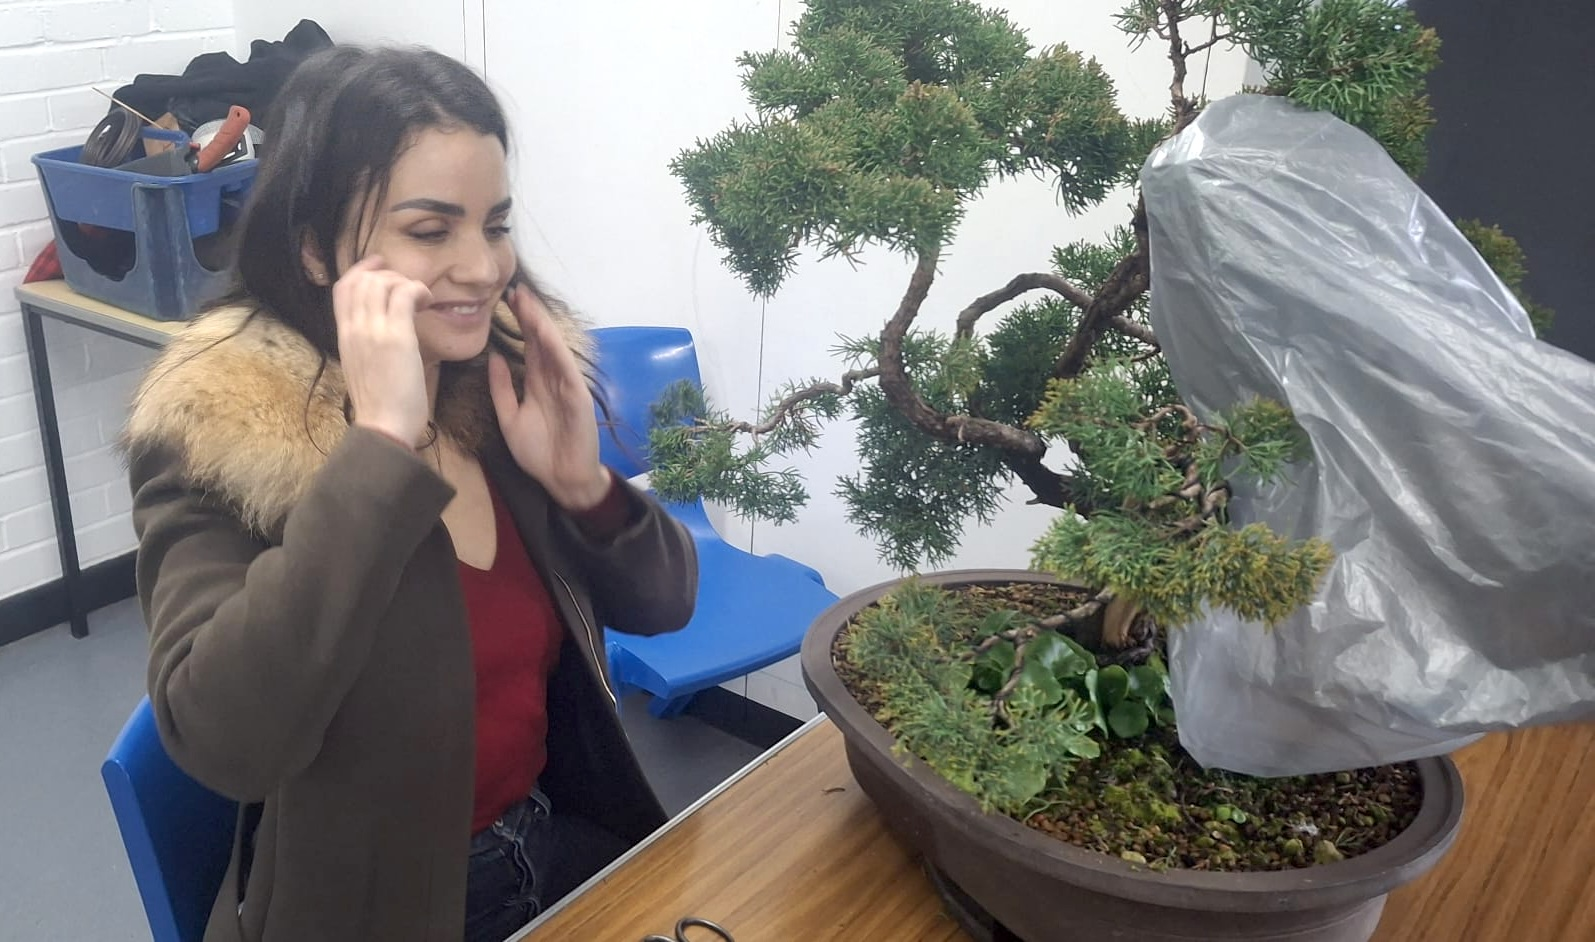
\includegraphics[angle=0,origin=c,width=1.0\textwidth]{2026_01/res/workshop_mep2_vistoria_training}
    \centerline{\emph{Victoria Miquel training for the New Talent Competition.}}
\end{minipage}

\begin{minipage}[b]{0.45\textwidth}
    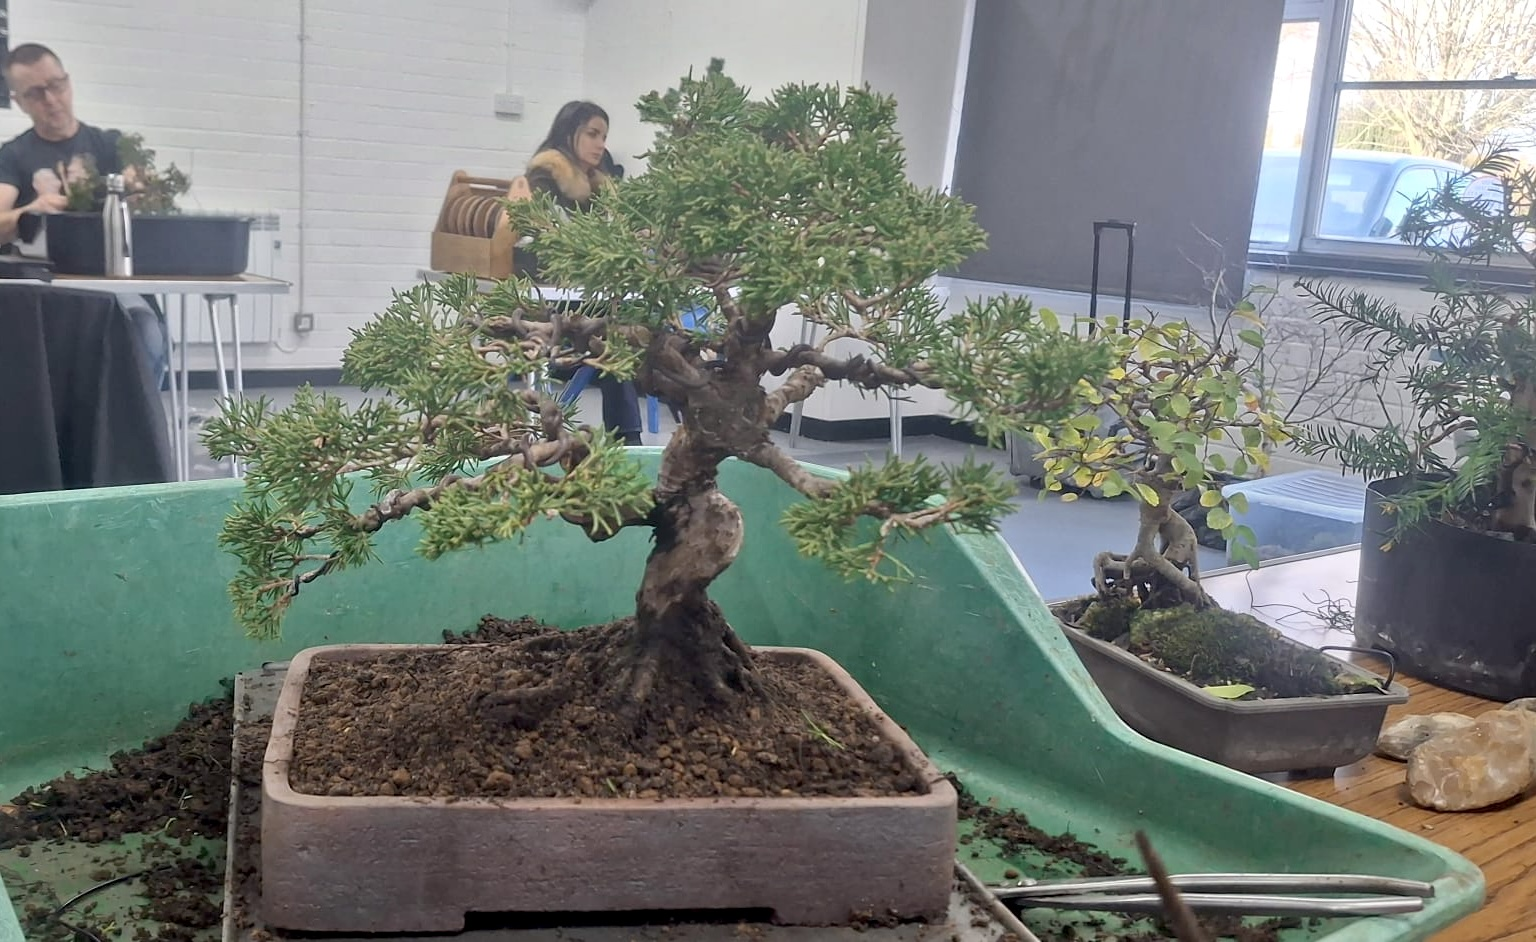
\includegraphics[angle=0,origin=c,width=1.0\textwidth]{2026_01/res/workshop_mep2_trees1}
    \centerline{\emph{One of the trees repotted during the session.}}
\end{minipage}

\columnbreak

\begin{minipage}[b]{0.45\textwidth}
    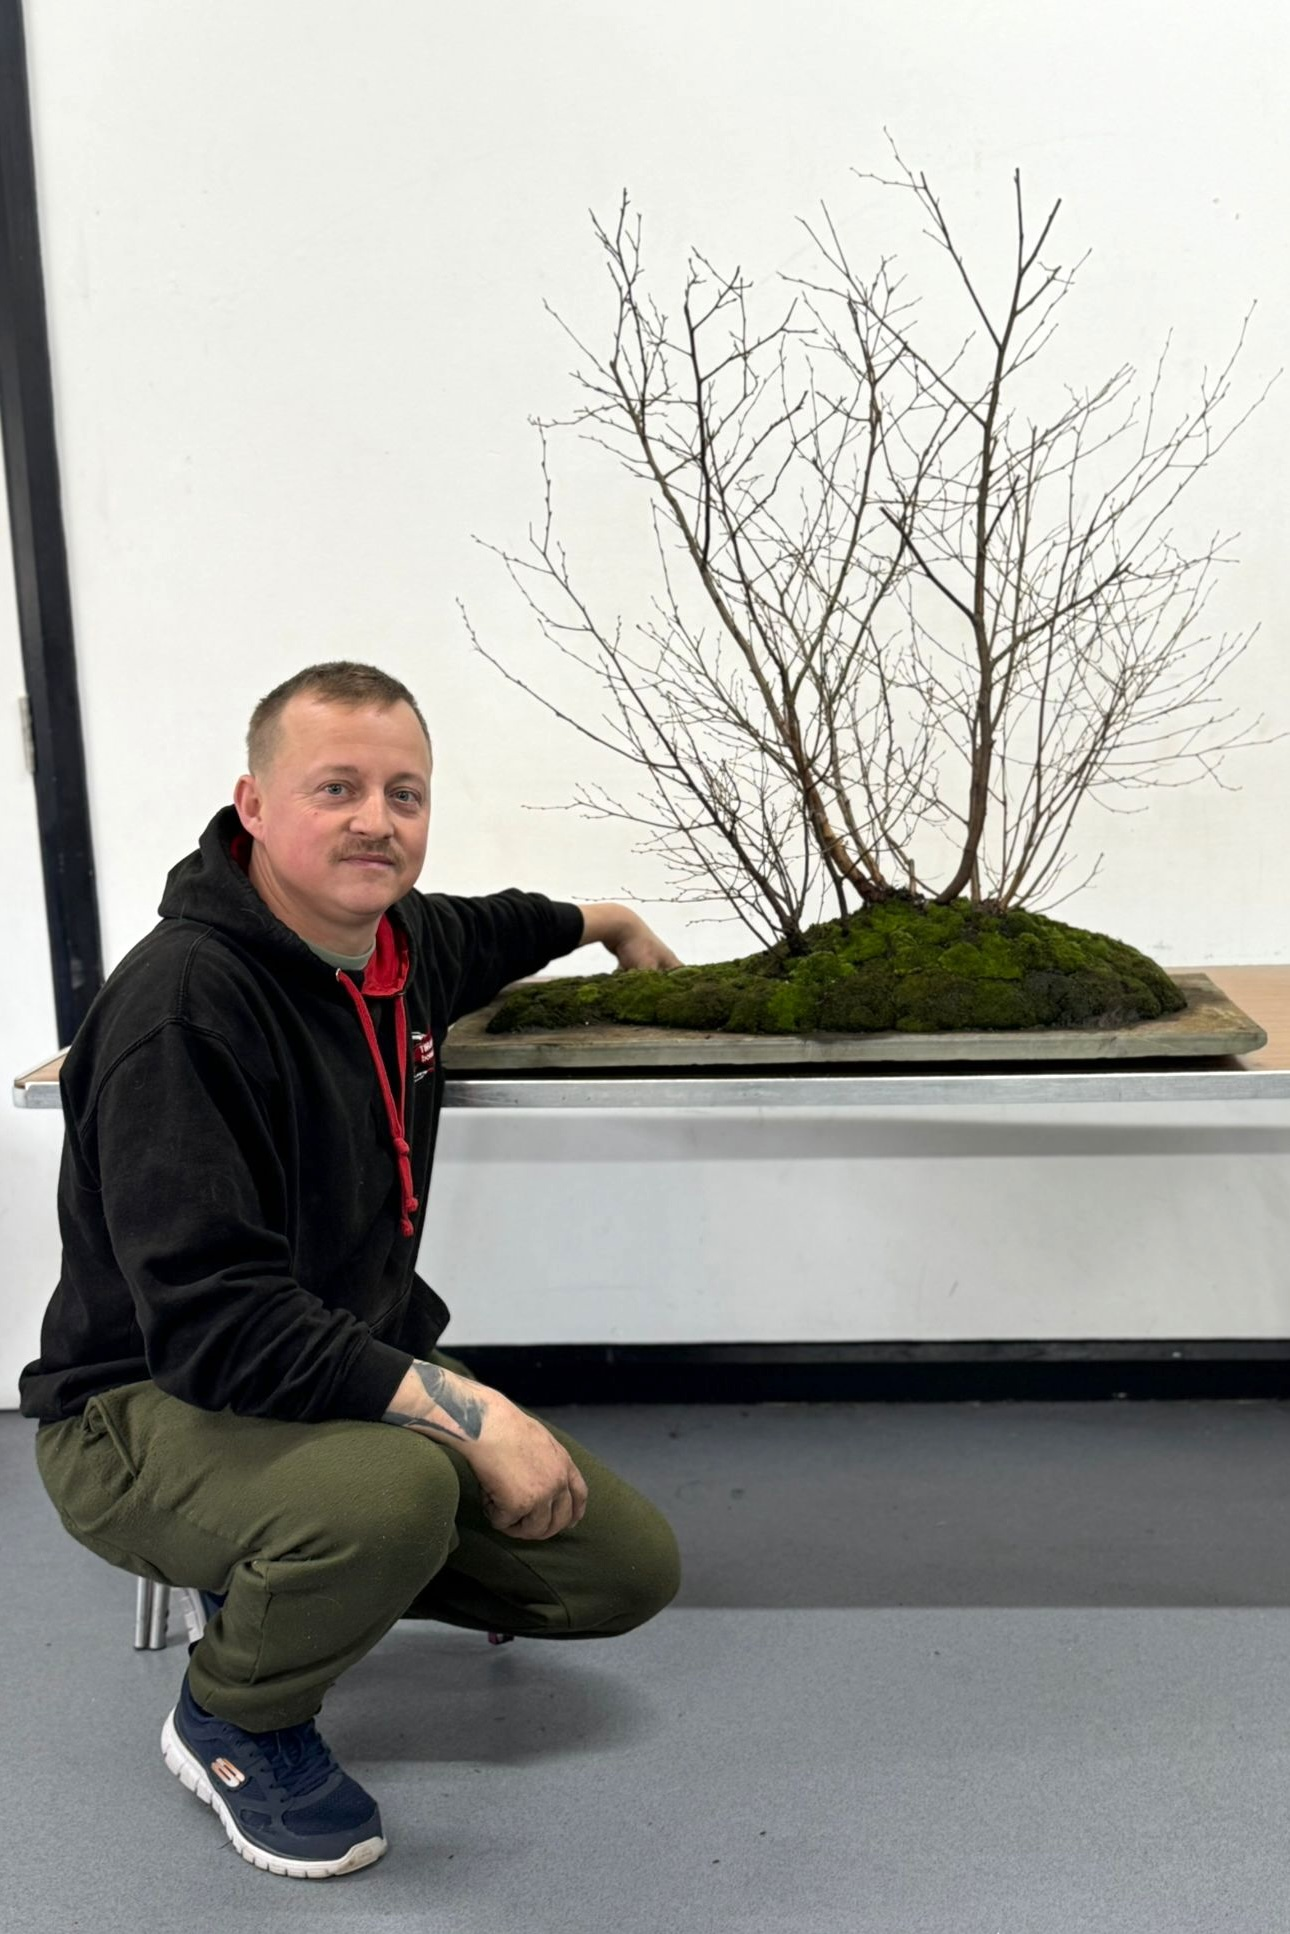
\includegraphics[angle=0,origin=c,width=1.0\textwidth]{2026_01/res/workshop_mep2_david_kabudachi}
    \centerline{\emph{David Fishwick's impressive birch clump on a slab.}}
\end{minipage}

\begin{minipage}[b]{0.45\textwidth}
    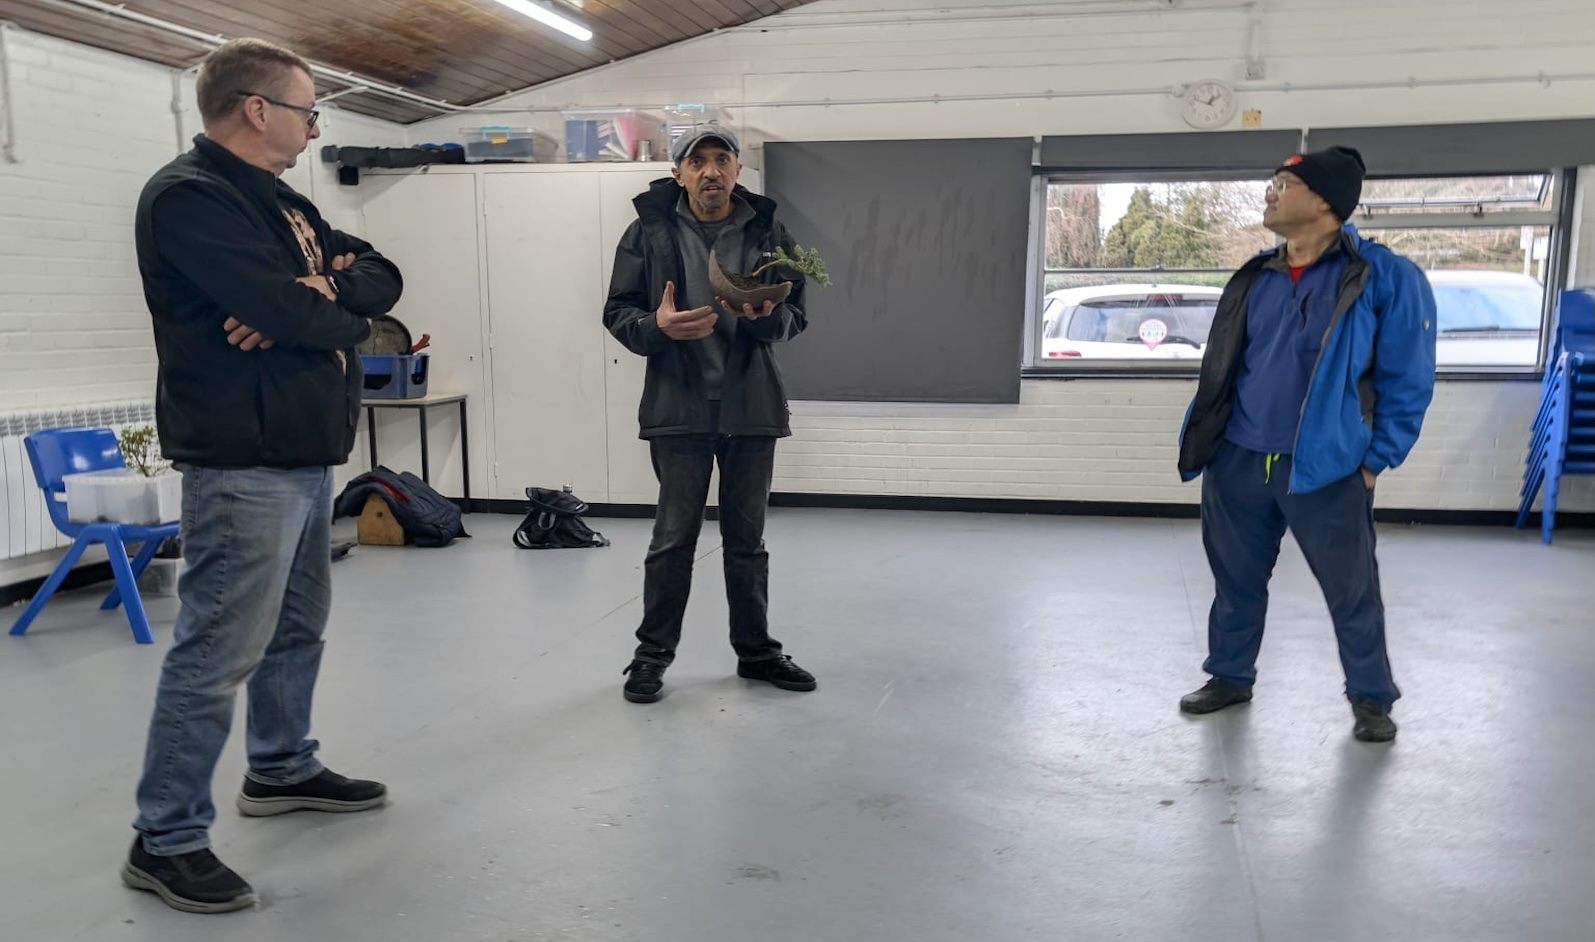
\includegraphics[angle=0,origin=c,width=1.0\textwidth]{2026_01/res/workshop_mep2_feedback}
    \centerline{\emph{The instructors and members during the feedback session.}}
\end{minipage}

\begin{minipage}[b]{0.45\textwidth}
    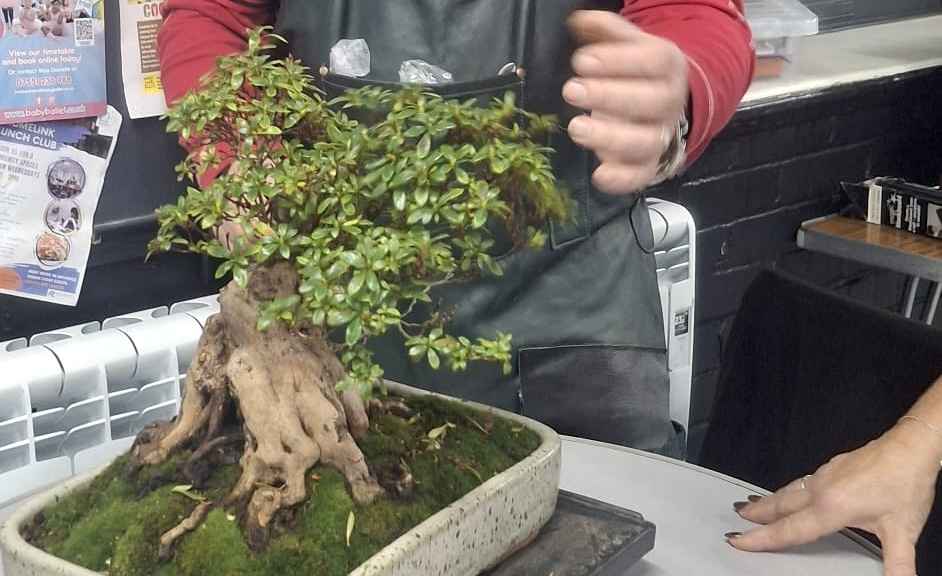
\includegraphics[angle=0,origin=c,width=1.0\textwidth]{2026_01/res/workshop_mep2_trees2}
    \centerline{\emph{Another tree receiving extra care during the session.}}
\end{minipage}

\columnbreak

